\chapter{Shapeshifters, Kappa and Tengu}

\section{Animal transformation}

Many Japanese yōkai are animals with the power to \emph{transform} (\ja{化ける},
bakeru), especially to take human form and deceive people. The power usually comes with
age: an animal that lives long enough acquires supernatural abilities.

\begin{center}
\begin{tabular}{lp{3.2cm}p{3.4cm}p{4.4cm}}
\toprule
Animal & Typical disguise & Character & Signature trick \\
\midrule
fox, kitsune \ja{狐} & beautiful woman & clever, seductive, sometimes divine & possession, fox-fire, illusions \\
raccoon dog, tanuki \ja{狸} & monk, kettle, merchant & jolly, foolish, lustful & leaf on the head to transform; belly drum \\
cat, bakeneko \ja{化け猫} & old woman, lady of a house & sinister, vengeful & licking lamp oil, reviving corpses \\
badger, mujina \ja{貉} & faceless person & trickster & the \emph{noppera-bō} prank \\
snake, hebi \ja{蛇} & woman & jealous, obsessive & coils around victims (Dōjōji) \\
\bottomrule
\end{tabular}
\end{center}

\section{Kitsune}

\subsection{Messenger and trickster}

Foxes have a double image in Japan:

\begin{itemize}
  \item \textbf{Divine}: foxes are the messengers of \textbf{Inari} (\ja{稲荷}), the kami of
        rice and prosperity. Inari shrines (about a third of all shrines in Japan, including
        Fushimi Inari in Kyoto with its thousands of red torii) are guarded by fox statues
        holding a key or a jewel in their mouths. Offerings include fried tofu (\emph{aburaage}),
        hence \emph{kitsune udon}.
  \item \textbf{Demonic}: foxes deceive, seduce and possess.
\end{itemize}

\begin{definition}[Kitsune-tsuki]
\emph{Kitsune-tsuki} (\ja{狐憑き}) is possession by a fox spirit, causing illness, strange
cravings (fried tofu) or erratic behaviour. Certain families were believed to keep foxes
(\emph{kitsune-mochi}) and were shunned. Meiji psychiatrists reclassified it as a mental
illness (Week 7).
\end{definition}

\subsection{Famous fox women}

\begin{itemize}
  \item \textbf{Kuzunoha} (\ja{葛の葉}): a white fox who marries a man and bears a son, the
        future Abe no Seimei. When discovered she leaves a poem: ``If you love me, come and
        visit me in the forest of Shinoda in Izumi'', the ``fox wife'' pattern.
  \item \textbf{Tamamo no Mae} (\ja{玉藻前}): the most beautiful woman at the court of
        retired Emperor Toba, who falls ill. The onmyōji (in many versions Abe no Yasunari)
        reveals her as a nine-tailed fox (\ja{九尾の狐}, kyūbi no kitsune) who had earlier
        ruined kings in India and China. She flees to Nasu, is killed by warriors and
        becomes the \emph{Sesshōseki} (``killing stone'') that poisons anything nearby.
\end{itemize}

\begin{remark}
The number of tails indicates age and power: a fox gains a tail every hundred years, up to
nine. The nine-tailed fox comes from Chinese tradition. The Pokémon Ninetales and the
nine-tailed fox in \emph{Naruto} draw directly on this.
\end{remark}


\section{Tanuki}

The \emph{tanuki} (\ja{狸}, often mistranslated ``raccoon'' or ``badger'') is a real canid,
\emph{Nyctereutes procyonoides}. Folklore tanuki are comic shapeshifters.

\begin{itemize}
  \item \textbf{Transformation}: they place a leaf on their head to change shape.
  \item \textbf{Belly drum}: on moonlit nights tanuki drum on their bellies
        (\ja{狸囃子}, tanuki-bayashi).
  \item \textbf{Bunbuku chagama} (\ja{分福茶釜}): a tanuki turns into a tea kettle, gets
        put on the fire, and ends up as a performing tightrope-walker who brings his owner
        wealth.
  \item \textbf{Statues}: the Shigaraki pottery tanuki outside restaurants and bars (straw
        hat, sake bottle, promissory note, big belly and very large testicles, a pun on
        good fortune) is a modern 20th-century icon.
\end{itemize}

\begin{center}
\begin{tabular}{p{3.5cm}p{4.8cm}p{4.8cm}}
\toprule
 & Kitsune & Tanuki \\
\midrule
Gender of disguise & usually female & usually male \\
Tone & elegant, dangerous, romantic & comic, bumbling, earthy \\
Religion & Inari messenger & mostly secular (some temple tanuki) \\
Folk saying & ``tricked by a fox'' & ``a tanuki's sleep'' (pretending) \\
Modern & \emph{Naruto}, Ninetales & \emph{Pom Poko} (Ghibli, 1994), Mario's tanooki suit \\
\bottomrule
\end{tabular}
\end{center}

\begin{example}[\emph{Pom Poko}]
Takahata Isao's 1994 Ghibli film shows tanuki using their transformation powers to fight
the development of Tama New Town outside Tokyo in the 1960s. Their tactics (including a
yōkai parade) fail; in the end some take human form and work as salarymen. The film turns
folklore into environmental and social critique and is full of Edo-style yōkai imagery.
\end{example}

\section{Bakeneko and nekomata}

\begin{itemize}
  \item A cat that lives long, grows large, or whose tail grows long may become a
        \emph{bakeneko} (\ja{化け猫}). One whose tail splits in two is a
        \emph{nekomata} (\ja{猫又}). Hence the old custom of docking cats' tails, and the
        prevalence of short-tailed Japanese bobtails in Edo prints.
  \item Bakeneko lick lamp oil (made of fish oil), stand on their hind legs, dance with a
        towel on their heads, reanimate corpses and take the shape of the women they kill.
  \item \textbf{Nabeshima bakeneko sōdō}: a 19th-century kabuki tale in which a cat
        avenges its mistress, killed by a lord of Saga, by taking her form and draining
        the lord's life. A cat as onryō.
  \item Contrast: the \emph{maneki-neko} (\ja{招き猫}, ``beckoning cat'') of shops is a
        good-luck cat. Cats, like oni, have been tamed.
\end{itemize}

\section{Kappa}

\begin{definition}[Kappa]
\emph{Kappa} (\ja{河童}, ``river child'') are water yōkai found in rivers and ponds
throughout Japan, with many regional names (\emph{kawatarō}, \emph{gataro},
\emph{kawaso}\ldots). They are child-sized, green or reddish, with a turtle-like shell,
webbed hands and feet, a beak, and a \textbf{dish} (\ja{皿}, sara) of water on top of the
head.
\end{definition}

\begin{center}
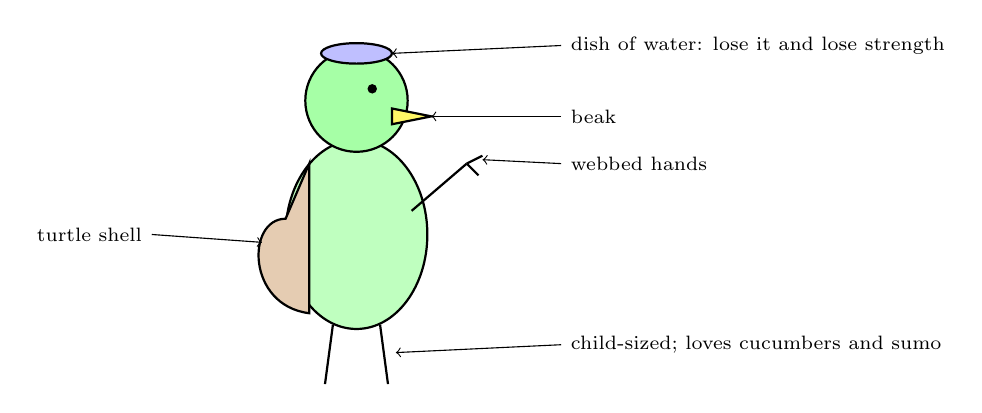
\begin{tikzpicture}[lab/.style={font=\scriptsize, align=left, anchor=west}]
  % body
  \draw[thick, fill=green!25] (0,0) ellipse (0.9 and 1.2);
  \draw[thick, fill=green!35] (0,1.7) circle (0.65);
  \draw[thick, fill=blue!25] (0,2.3) ellipse (0.45 and 0.13);
  \draw[thick, fill=yellow!60] (0.45,1.6) -- (0.95,1.5) -- (0.45,1.4) -- cycle;
  \fill (0.2,1.85) circle (0.06);
  \draw[thick, fill=brown!40] (-0.9,0.2) .. controls (-1.4,0.2) and (-1.4,-0.9) .. (-0.6,-1.0) -- (-0.6,0.9) -- cycle;
  \draw[thick] (0.7,0.3) -- (1.4,0.9); \draw[thick] (1.4,0.9) -- (1.6,1.0); \draw[thick] (1.4,0.9) -- (1.55,0.75);
  \draw[thick] (-0.3,-1.15) -- (-0.4,-1.9); \draw[thick] (0.3,-1.15) -- (0.4,-1.9);
  % labels
  \draw[->] (2.6,2.4) node[lab] {dish of water: lose it and lose strength} -- (0.45,2.3);
  \draw[->] (2.6,1.5) node[lab] {beak} -- (0.95,1.5);
  \draw[->] (2.6,0.9) node[lab] {webbed hands} -- (1.6,0.95);
  \draw[->] (-2.6,0.0) node[lab, anchor=east] {turtle shell} -- (-1.2,-0.1);
  \draw[->] (2.6,-1.4) node[lab] {child-sized; loves cucumbers and sumo} -- (0.5,-1.5);
\end{tikzpicture}
\end{center}

\subsection{What kappa do}

\begin{itemize}
  \item Drag people and horses into water to drown them; steal the \emph{shirikodama}, a
        mythical ball in the anus believed to hold one's soul.
  \item Challenge passers-by to sumo. Since kappa are scrupulously polite, the trick is to
        bow: the kappa bows back, spills the water from its dish and loses its strength.
  \item Love cucumbers (hence \emph{kappa-maki} sushi rolls); people throw cucumbers with
        their names into rivers to avoid drowning.
  \item When captured, a kappa may promise never to harm the village again, or teach the
        art of setting bones, a ``kappa deed'' (\ja{河童の詫び証文}).
\end{itemize}

\begin{important}[Interpretations]
\begin{itemize}
  \item \textbf{Fallen water god}: Yanagita saw kappa as degraded river deities who once
        received offerings (cucumbers as first fruits).
  \item \textbf{Drowning}: kappa explain drownings of children and are a warning to stay
        away from rivers. Some scholars connect kappa legends to the bodies of children lost
        in floods or to infanticide (\emph{mabiki}).
  \item \textbf{Outsiders}: some legends link kappa to marginalized groups who worked on rivers.
  \item \textbf{Modern mascots}: the Kizakura sake kappa; Akutagawa Ryūnosuke's satirical
        novel \emph{Kappa} (1927); the cute kappa of \emph{Summer Days with Coo} (2007).
\end{itemize}
\end{important}

\section{Tengu}

\begin{definition}[Tengu]
\emph{Tengu} (\ja{天狗}, ``heavenly dog'', from a Chinese term for a meteor) are mountain
yōkai. Early tengu were bird-like (\emph{karasu-tengu}, ``crow tengu'', with beaks and
wings); from the medieval period the familiar tengu has a \textbf{red face and a long nose}
(\emph{hanadaka-tengu}), wears the clothes of a \emph{yamabushi} mountain ascetic, and
carries a feather fan.
\end{definition}

\begin{itemize}
  \item \textbf{Buddhist enemies}: in medieval tales tengu are the spirits of arrogant monks
        who could not achieve enlightenment and now obstruct Buddhism; the ``tengu realm''
        (\ja{天狗道}) is a kind of extra Buddhist hell for the proud. ``To become a tengu''
        (\ja{天狗になる}) still means to become conceited.
  \item \textbf{Kidnappers}: children who vanished in the mountains were said to have been
        ``hidden by the kami'' (\ja{神隠し}, kamikakushi; compare \emph{Spirited Away},
        Week 11) or taken by tengu. The Edo scholar Hirata Atsutane interviewed a boy,
        Torakichi, who claimed to have lived with tengu.
  \item \textbf{Martial arts teachers}: the tengu Sōjōbō of Mount Kurama taught swordsmanship
        to the boy Minamoto no Yoshitsune.
  \item \textbf{Mountain gods}: in mountain worship (\emph{shugendō}) tengu are protector
        spirits; tengu masks are sold at mountain temples such as Takaosan.
\end{itemize}

\begin{center}
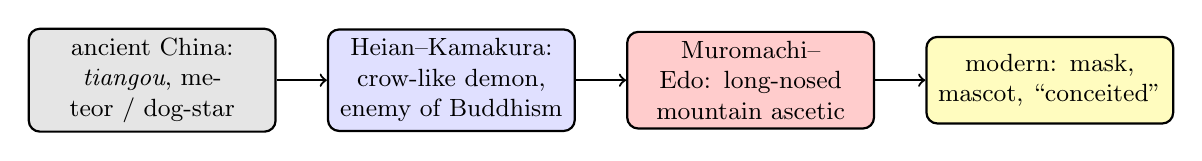
\begin{tikzpicture}[b/.style={draw, thick, rounded corners, align=center, font=\small, text width=2.9cm, minimum height=1.1cm}]
  \node[b, fill=gray!20] (a) at (0,0) {ancient China:\\\emph{tiangou}, meteor / dog-star};
  \node[b, fill=blue!12] (b) at (3.8,0) {Heian--Kamakura: crow-like demon, enemy of Buddhism};
  \node[b, fill=red!20] (c) at (7.6,0) {Muromachi--Edo: long-nosed mountain ascetic};
  \node[b, fill=yellow!25] (d) at (11.4,0) {modern: mask, mascot, ``conceited''};
  \draw[->, thick] (a) -- (b); \draw[->, thick] (b) -- (c); \draw[->, thick] (c) -- (d);
\end{tikzpicture}
\end{center}

\section{Taxonomy of this week's creatures}

\begin{center}
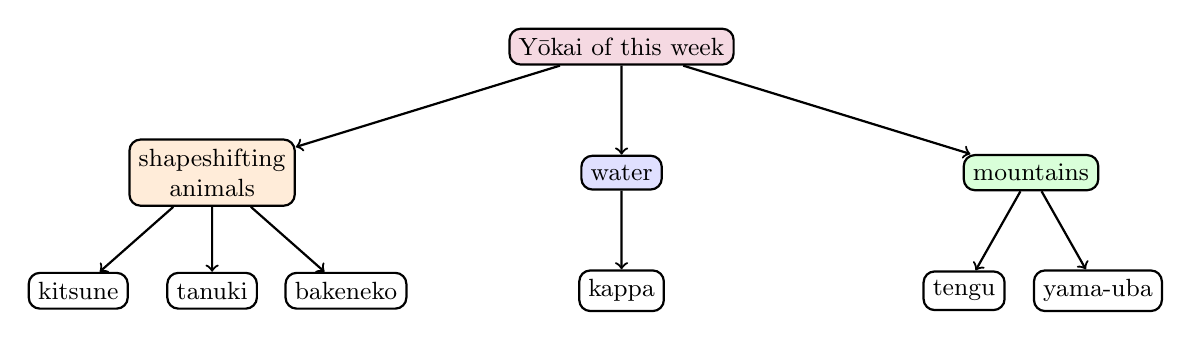
\begin{tikzpicture}[
    level 1/.style={sibling distance=5.2cm, level distance=1.6cm},
    level 2/.style={sibling distance=1.7cm, level distance=1.5cm},
    every node/.style={draw, thick, rounded corners, align=center, font=\small, fill=white},
    edge from parent/.style={draw, thick, ->}]
  \node[fill=purple!15] {Yōkai of this week}
    child { node[fill=orange!15] {shapeshifting\\animals}
      child { node {kitsune} }
      child { node {tanuki} }
      child { node {bakeneko} } }
    child { node[fill=blue!12] {water}
      child { node {kappa} } }
    child { node[fill=green!15] {mountains}
      child { node {tengu} }
      child { node {yama-uba} } };
\end{tikzpicture}
\end{center}

\section*{Summary}
\begin{itemize}
  \item Long-lived animals gain the power to transform: kitsune (elegant, seductive, also
        Inari's messengers), tanuki (comic), bakeneko/nekomata (sinister cats).
  \item Kitsune possession, fox wives (Kuzunoha) and the nine-tailed Tamamo no Mae.
  \item Kappa: river yōkai with a water-dish, cucumbers and sumo; read as fallen water
        gods and as explanations for drowning.
  \item Tengu: from Chinese meteor-dog to crow demon to long-nosed mountain ascetic.
\end{itemize}
